\documentclass[twocolumn]{article}
\usepackage{color}
\usepackage{listings}
\usepackage{float}
\usepackage{amsfonts}
\usepackage{amssymb}
\usepackage{amsmath}
\usepackage{cite}
\usepackage{listings}
\usepackage{xcolor}
\usepackage{graphicx}
\usepackage{draftwatermark}
\SetWatermarkText{DRAFT YELLOW PAPER}
\SetWatermarkScale{1}
\definecolor{pagecolor}{rgb}{1,0.98,0.9}
\pagecolor{pagecolor}
\setlength\parskip{.5\baselineskip}
\author{Ryan J. Kung \\ryankung@ieee.org\\Member, IEEE Blockchain Community }
\title{Inferred based Distributed Gaming, Nash Equilibrium}
\begin{document}
\maketitle
% \tableofcontents
\section{Abstract}

Since the introduction of Ethereum on 2014\cite{ethereum}, It brought many DApps and DGames, such as CryptoKitty, Etheremon and Decentraland. Most of them were running into issues addressed to the congestion of transaction which is limitation of how Ethereum implemented. Storing on-chain data is too expensive for games needs high interaction, and may cause may problem, one of them is that gaming on distributed system may cause harder to find out a fear nash equilibrium point for numerical designing, and the nonnegligible delay of tranasction caused may limited the interactive rate of game processing.

In this paper, we studied and discussed how should a distributed game works on blockchain based distributed system. First, we discussed distributed nash equilibrium problem on certain condition, then we introduced an infered based system based on an abstraction which formalize blockchain with STMonad and Lens application, further, we discussed how to composed infered system with zero-knowledge proof for game refining.

\section{Distributed Nash-Eq}

Like traditional Gaming on game theory, we defined DGaming as a series of Gaming Behaviors and Strategis which is Distributed. With Lamport's defination on 1978\cite{time-clocks-ordering-events-distributed-system}, A Gaming is Distributed if the message transaction delay is not negligible compared to the time between event in classic gaming behavior. The issues in traditional gaming theory may easily lead us run into trouble if it's distributed, such as nash equilibrium simulation or prisoner's dilemma problem.

On classic Nash Equilibrium, we seeking out the nash-eq point by analyze it with action matrix, and proof that for each strategy on game $(S, f)$, and got A strategy profile which is Nash Equilibrium. But on distributed case, the issue is that the event of strategy is not effect immediately, nonnegligible delay of transaction on system may cause N-Eq point out of expectation.

For example, we discuss a classic game as:
\begin{center}
\begin{tabular}{c|c|c|}
  & L & R \\
  \hline
  U & (1,3)&(-3,0)\\
  \hline
  M & (-2,0)&(1,3)\\
  \hline
  D & (0,1)&(0,1)\\
\end{tabular}
\end{center}

With Repeated advantage solution, we can simply figure out that the nash-eq strategy is $(U, L)$, but this game is based on a hypothesis that player $i$ shares same knowledge about payoff and strategy space. If players are sensitive on the uncertainty of $s_{-1}$, they may not choose the rational strategy, like if about \%1 players choose $R$, then $D$ is better than $U$.


\begin{figure}[H]
  \centering
  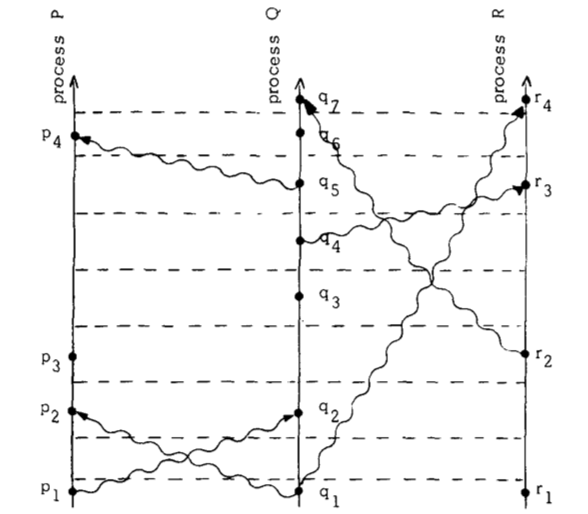
\includegraphics[width=0.5\linewidth]{img/lamportts.png}
  \caption{Lamport Timestamp}
\end{figure}


In distributed game, for example an distributed game based on a paxos based system. Addressed to the nonnegligible delay, player $i$ may upfront know $i'$ and action hysteretic, which may cause the nash-equilibrium become highly dependents on the distributed network. Figure 1 is showing that how events can be trigger and measured on a distributed system. Actually, on a Dgame all players may tried to mining more informations and action as later as they can, the situation may looks like Prisoners’ Dilemma:

\begin{center}
\begin{tabular}{c|c|c|}
  & W & A \\
  \hline
  W & (1,1)&(-1, 2)\\
  \hline
  A & (2,-1)&(0,0)\\
\end{tabular}
\end{center}

On this game, players can choose from strategy space ${Wait, Action}$, and as what prisoner's dilemma presented to us, all players may choose $W$. Which entangled the gaming into a series complicated case, and break perfect information gaming in to imperfect.Actually, Nash equilibrium seeking under communication networks is as tracing increasing attension resently, Some seeking work is about paritially coupled payoff method\cite{8029164}, or Communication Topologies\cite{8093754}. In this paper, we considered distributed Nash equilibrium with a set of player $\mathbb{N} = {1, 2, ..., N}$, under a distributed network which has nonnegligible delay $\mathbb{\delta}$, and Denote $f_i(x)$ as the payoff function of player $i$, where $X = [x_1, x_2, ..., x_n]^T$, $x_i \in S$ is action of player i. And we define a measurement function $m = f(\delta, i)$ which is means how the information is prefect for player $i$.

The distributed equilibrium seeking strategy(DESS) was given by \cite{7888532}:
\begin{gather}
  \dot{x} = k_i \frac {\partial f_i}{\partial x_i}(y_i), i \in \mathbb{N}
\end{gather}

$(\dot{x}^*, 1_N\oplus x^*)$, where $x^*$ presents nash equilibrium. There are some descendent work based on it, but most of them are analytically studied based on certain condition, ignores nonnegligible communication or transaction cost, which is non-ignorable in blockchain and other distributed system. In blockchain case, we can compose measurement function and DESS together, then the strategy can be present as $m(\delta, \dot{x})$. And obviously, there should be existed some relationship between Nash-eq point and $\delta$, such as:

\begin{gather}
  m(\delta_a, \dot{x}) > m(\delta_b, \dot{x}) \vdash a > b
\end{gather}

\section{Infered information}

Unlike classic distributed system,
Since some formalization of blockchain is based on the separation logic or $\pi calculis$ \cite{linearblockchain}, it can easily be modeled as a time step function, or a FRP issue which can be abstract as\cite{ElliottHudak97:Fran}, where blockchain Status can be also be abstract as $STMonad$ like MAKERDao\cite{dai}'s work:

\begin{gather}
  time: STMonad_{time}\\
  at \mathbb{[} time \mathbb{]}t = t
\end{gather}

Unlike other issues we met in pure functional world, there should be only one types of monad in blockchain, the STMonad, $STMonad$ is a Monad type for status, thus except status changes, all other functions should be pure which means no side-effect, which means we can build an infered system or a $LENS$\cite {lens} above it. A Lens should have two property, $over$, and $view$. 

\lstset{language=Haskell}
\begin{lstlisting}
data Lens a b = Lens
    { view :: a -> b
    , over :: (b -> b) -> (a -> a)
  }
\end{lstlisting}

A concrete example based on Solidity is, for each functions, if it's a pure function which means nor cost gas or cause side-effect on blokchain it can be infered based on ABI, it's a $view$, otherwise it's a $over$ which means you have to send a transaction to modified the status of chain. From $(2)$ we know that the distributed nash-equilibrim point is based on the transaction param $\delta$, thus we can assume that $Lens.view$, and $Lens.over$ is some paritial function based on $\delta$. We know that if $view$ is a pure function so that $\lim \delta$ is 0, which means if a client is well connected to the network, the $\delta$ is negligible for that, since for $over$ case, you can only shift $\delta$ by provide a high $tranasction\ price$ (gas price for ethereum).


So since classic distributed gaming may transfer the gaming from perfect information to imperfect. But if it's blockchain based, since $over$ is working as eventual consistency\cite{consis} but the status of blockchain can be seems as strong consistency\cite {Consistent}. On $view$ phase of gaming, when player $i$ make decision on $STMonad time_0$, the information of $Monat$ is perfect. For phase $over$, players may choose to pay high price as strategy to get more payoff, since it's based on consistency information of blockchain, we can also say that the $over$ phase is also perfect information gaming. So for a gaming we wished to have a fixed nash equilibrium point, it should be designed as all data in public and no private status.

\section {Zero Knowledge Gaming}

Such as we can formalize blockchain as a Monad (A monoid in the category of endofunctors), We can also describe abstractly the cryptology part of bitcoin as a cyclic subgroup of elliptic curve group over a primer finite field, which is also the the key of zk-SNARKs. There is an concrete implementation in our game for providing zero-knowledge proofing based on the infered system and hash algorithms, It's works like other blockchain implementation does \cite{zcash}. But what further more is, we tried developed algorithms based on Abstract Algebra Type and Isomorphism or Bijection mapping.

The Abstract Algebra Type made an allowance for playing high abstract part of calculators in a more intuitionistic way. Such as when we try to implement ethereum's pubkey/privatekey algorithm, we can just simply write as\cite{klefki}:

\lstset{language=Python}
\begin{lstlisting}
  def pubkey(priv: CF) -> ECG:
      return ECG(G @ priv)
\end{lstlisting}

Where CF and ECG is Finite Field Cyclic Group and Elliptic Curve Group of Secp256k1. By the property of cyclic subgroup, we can easily improve the zero knowledge gaming as some endomorphism feature.

\begin{gather}
  A + B = X \\
  A + C = X \\
  C \neq X
\end{gather}

\section {More Concrete}

In the Go!hamster, the game we designed based on this work. We abstract the gaming activity as mining, and designed a series of numerical system, which can maintain the value of user actor by a fixed and well-designed nash equilibrium pointed. 
\subsection {Decentralized Marking}

The ERC20 standard was extended with a built-in transparen exchange, which makes all gaming actor can be limited inside the blockchain or contract. And based on ERC721, we designed a reward system to keep player can get payoff if they act around the nash-eq point. For Exchangeable ERC20 and so on the Exchangeable ERC721, all matching stuffs is based on infered system, which means players can check the full depth of ticker for determining the best price they should pay for tokens.

Functions of smart contract are separated into Functor and Monad. Functors are working based on pre-infered system, and Monads are based on infered system, which is actually presented a sequence of status.

\subsection {Infered Token Balance}

On out implementation of Gaming Token, we designed an infered based auto expended rate. The expended rate is based on $\delta$ and $time$ of blockchain, which is bounded on the nash equilibrim of what the token price should be during the game processing.

\subsection {Gaming Versus Mining}

The most obviously case of nash-eq case on blockchain world is bitcoin mining\cite{bitcoin}, we can easily build an game matrix model on bitcoin mining behavior, the relationship is between market force, difficult rate, and hash rate. And in game Go!hamster, actors can pay game token for wining reward, more token they paid, higher rewarding rate they got, which is working as a simulation of how bitcoin mining works.

\section {Conclusion}

Addressed to the strong consistency property of blockchain, A game can have a certain nash equilibrium point, if the side-effects and pure-functions are in separation. Though there is alot of limitation on Ethereum and solidity itself, a real-time game, like RPG or Action game can be still build on a monad based and zero-knowledge based infered system.

\bibliographystyle{plain}
\bibliography{dgaming}
\end{document}
